\documentclass[tikz,border=5]{standalone}
\usepackage{tikz}
\usetikzlibrary{%
    decorations.pathreplacing,%
    decorations.pathmorphing,
    decorations.markings%
}
\usetikzlibrary{patterns,calc,arrows}
\usepackage{pgfplots}

%% please note changes in color %%
% base color for copper and PCB
\definecolor{copper}{rgb}{1,0,0}
\definecolor{pcb}{rgb}{0,1,0}
% shades of them for the different elements
\colorlet{groundplane}{copper!50!black}
\colorlet{pcbfront}{pcb!50!black}
\colorlet{pcbright}{pcb!20!black}
\colorlet{pcbtopleft}{pcb!70!black}
\colorlet{pcbtopright}{pcb!50!black}
\colorlet{striplinefront}{copper!50!black}
\colorlet{striplineright}{copper!50!black}
\colorlet{striplinetopleft}{copper!90!black}
\colorlet{striplinetopright}{copper!60!black}

\begin{document}

\pgfarrowsdeclarecombine{dimarrow}{dimarrow}{latex}{latex}{}{}
\def\Dimline[#1][#2][#3]{
        \draw[ % |-|, % removed, looks odd for l
        decoration={markings, % switch on markings
                mark=at position 0 with {\arrowreversed[scale=0.5]{dimarrow}};,
                mark=at position .5 with {\node[black] at (0,0.25) {#3};},
                mark=at position 1 with {\arrow[scale=0.5]{dimarrow}};,
            },
        postaction=decorate] #1 -- #2 ;
}

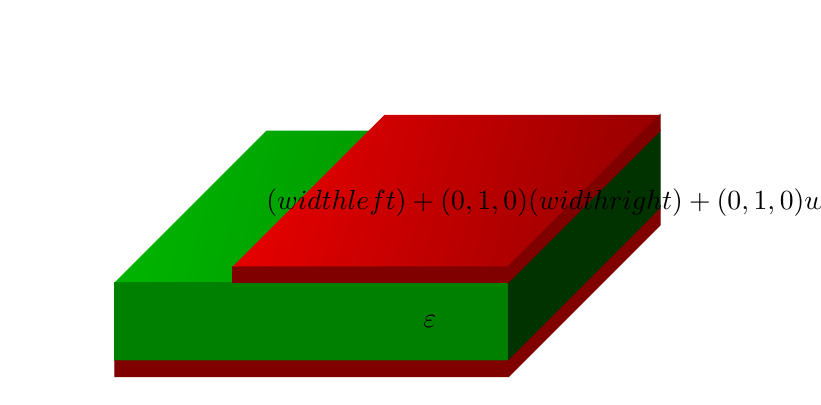
\begin{tikzpicture}

% PCB front, use cycle to close path
\filldraw [pcbfront] (0,0,5) coordinate (height bottom) -- (0,1,5) coordinate (height top) -- (5,1,5) -- (5,0,5) -- cycle;

% PCB top
\shade[top color = pcbtopleft, bottom color = pcbtopright, shading angle=75] (0,1,0) -- (5,1,0) -- (5,1,5) -- (0,1,5) -- cycle;

% PCB right, closed it
\filldraw [pcbright] (5,0,0) -- (5,0,5) -- (5,1,5) -- (5,1,0) -- cycle;

% groundplane
\filldraw [groundplane] (0,0,5) -- (5,0,5) -- (5,0,0) -- (5,-0.2,0) -- (5,-0.2,5) -- (0,-0.2,5) -- cycle;

% stripline front
\filldraw [striplinefront] (1.5,1.2,5) coordinate (length front) -- (5,1.2,5) coordinate (thickness top) -- (5,1,5) coordinate (thickness bottom) -- (1.5,1,5) -- cycle;

%stripline top
\shade [top color = striplinetopleft, bottom color = striplinetopright, shading angle=75] (1.5,1.2,0) coordinate (width left) coordinate (length back) -- (5,1.2,0) coordinate (width right)  -- (5,1.2,5) -- (1.5,1.2,5) -- cycle;

% stripline right
\filldraw [striplineright] (5,1,5) -- (5,1.2,5) -- (5,1.2,0) -- (5,1,0) -- cycle;

\node at (4,0.5,5) {$\varepsilon$};


% stripline width
\Dimline[($(width left)+(0,1,0)$)][($(width right)+(0,1,0)$)][$w$];
\draw ($(width left)+(0,0.1,0)$) -- ($(width left)+(0,1.1,0)$);
\draw ($(width right)+(0,0.1,0)$) -- ($(width right)+(0,1.1,0)$);

% stripline length
\Dimline[($(length back)+(-2.5,0,0)$)][($(length front)+(-2.5,0,0)$)][$l$]; %[left];
\draw ($(length front)+(-0.1,0,0)$) -- ($(length front)+(-2.6,0,0)$);
\draw ($(length back)+(-0.1,0,0)$) -- ($(length back)+(-2.6,0,0)$); 

% stripline thickness
\Dimline[($(thickness top)+(3.5,0,0)$)][($(thickness bottom)+(3.5,0,0)$)][$t$]; %[left];
\draw ($(thickness top)+(0.1,0,0)$) -- ($(thickness top)+(3.6,0,0)$);
\draw ($(thickness bottom)+(0.1,0,0)$) -- ($(thickness bottom)+(3.6,0,0)$);      

% PCB height
\Dimline[($(height top)+(-1,0,0)$)][($(height bottom)+(-1,0,0)$)][$h$]; %[left];   
\draw ($(height top)+(-0.1,0,0)$) -- ($(height top)+(-1.1,0,0)$);
\draw ($(height bottom)+(-0.1,0,0)$) -- ($(height bottom)+(-1.1,0,0)$);

\end{tikzpicture}

\end{document}